\documentclass[12pt]{article}
\usepackage{fullpage}
\usepackage[top=2cm, bottom=4.5cm, left=2.5cm, right=2.5cm]{geometry}
\usepackage{fancyhdr}
\usepackage{graphicx}

\pagestyle{fancyplain}
\headheight 35pt
\lhead{Aidan Bush, David Dowie, Ben Ha}
\rhead{CMPT 355 \\ \today}
\headsep 1.5em

\begin{document}

\section*{Project 2-Konane}

\subsection*{Implementation}
In our approach we used Alpha-Beta pruning with iterative deepening.
Iterative deepening was used so that we are able better work within the time limit.
The iterative deepening also resulted in our agent in exploring an entire depth of possible moves.
We also sorted potential moves by their evaluation values to allow for Alpha-Beta pruning.

% timing
To time our agent, and ensure It had a move in the time allotted we used a separate thread with a timer.
Before we started our search for each move we would create the thread to be our timer.
The thread would sleep for the time allotted for the move, and then would wake up and set a flag to signify that the time was up.
The search would check the timer flag and then recurse back out of the iterative deepening loop before printing off the move.

To represent our state space we used a multi-dimensional array of 8 by 8 one byte integers.
We used this model to allow easy access to each of the boards entries, and to simplify development.

\subsection*{Enhancements}
% saving moves
To improve out approach we kept all moves throughout our successive moves.
This allowed us to not have to re-search all the moves we had for our previous moves.
Saving moves also allowed us to search deeper that if we had not as we would continue off on the search we stopped on.
Specifically the agent would start searching at 3 less than the depth we stopped, to account for our, and our opponents move, and then would continue off on the last depth we were searching at.
This improvement did have a downside, in that we would always generate all possible moves from a specific depth.
If we did not we would have to constantly check for moves we left out when searching for our next move.
Although this could be done in the time our opponent spent making a move.

% timer in separate thread
We implemented our timer in a separate thread from our main search.
Using a second thread made checking the time easier, as we could just used a flag that would be set when the time was up.
Using the flag resulted in searching though more moves and finding better moves, along with winning moves quicker.
The second thread also slept which meant that it would not take up time from our main thread.

% compiler optimization
We introduced compiler optimization though the -O3 optimization flag.
Using compiler optimization improved performance of the agent allowing it to explore many more moves.

\subsection*{Performance}
We ran tests on Aidan's laptop to generate statistics on it running, which ran faster than the student server.

Figure~\ref{fig:explore} shows the number of nodes explored per turn.
This number is not necessarily the number of new nodes explored.
The jump at the end is caused by our agent revisiting many nodes as it had explored all possible moves from that point.

Figure~\ref{fig:create} shows the number of nodes created per turn.
This is the number of new nodes that are created, at the end of the games it reaches 0 as all possible moves have been created.

Figure~\ref{fig:depth} shows the maximum depth the agent reached per turn.
Near the end when the agent reached all possible moves had been created the agents max depth starts to dip.

\begin{figure}
  \centering
  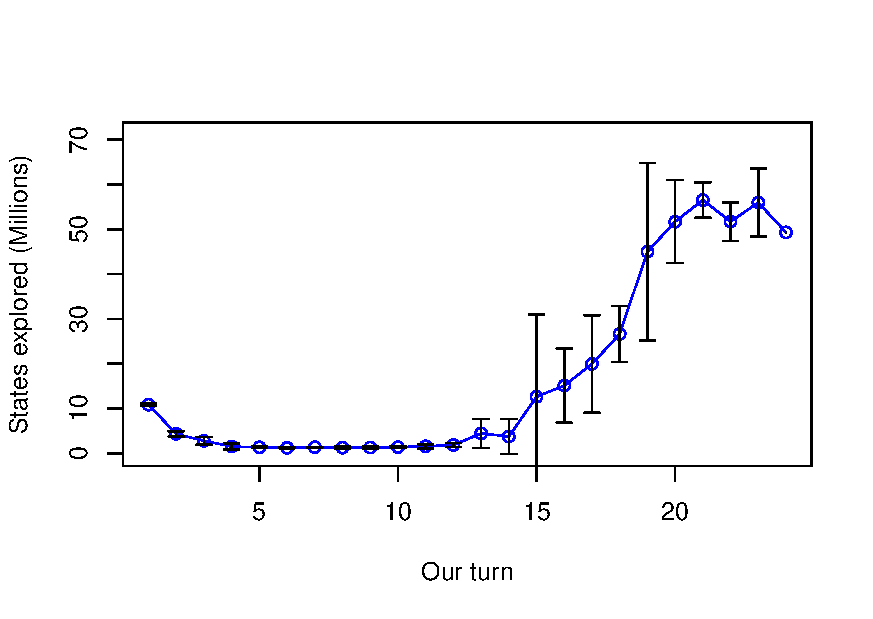
\includegraphics[scale=0.5]{../results/explored_plot.pdf}
  \caption{Plot of explored nodes for each turn.}
  \label{fig:explore}
\end{figure}

\begin{figure}
  \centering
  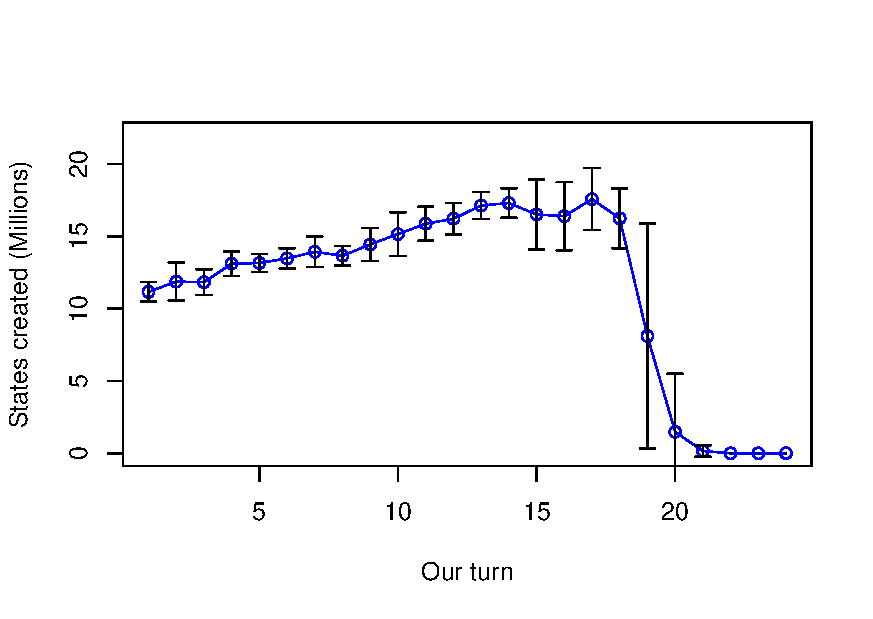
\includegraphics[scale=0.5]{../results/created_plot.pdf}
  \caption{Plot of created nodes for each turn.}
  \label{fig:create}
\end{figure}

\begin{figure}
  \centering
  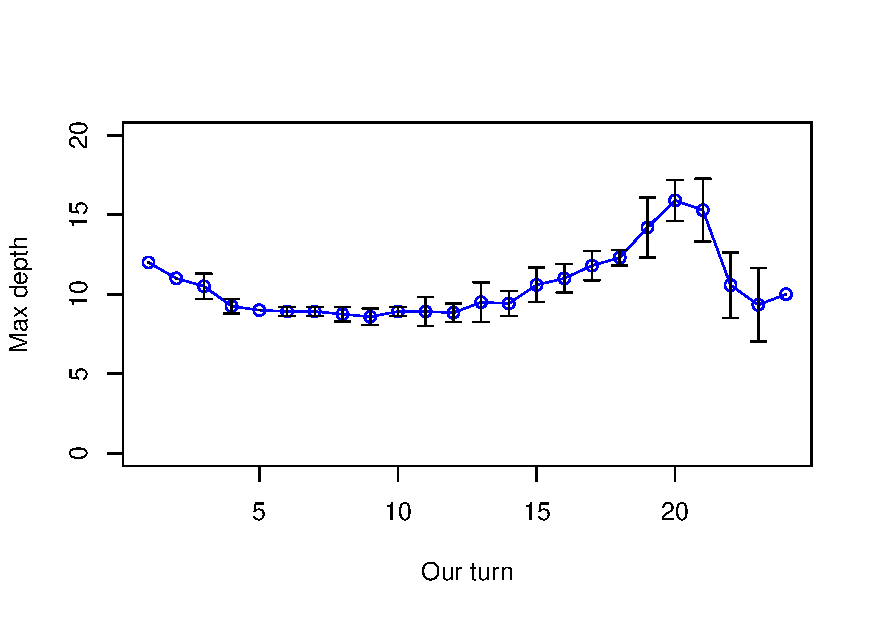
\includegraphics[scale=0.5]{../results/depth_plot.pdf}
  \caption{Plot of max depth reached for each turn.}
  \label{fig:depth}
\end{figure}

\subsection*{Problems}
% printing off and selected differing moves
To ensure that we printed a valid move within the given decision making time we opted into printing the top move move the instant our thread sleep was completed.
We also wanted to always sort the children of each state so that for max they are sorted in decending order and for min in ascending order.
Since we sorted these nodes recursively, we were printing the state at children[0].
Therefore we were not actually printing the best move for the given state.
To fix this we changed our base case to be when; we found a end game state, we reached our specified max depth, or when the time is up.
We then printed the move after the alpha-beta algorithm was completed leaving us with the most optimal move, based off our search,  every time.

% missed leftmost column and topmost row moves
Another problem we had was generating moves which required a jump that ended in either the top-most row or the left-most column.
We were simply just not evaluating the state properly by looking at every index greater than zero for either left or up moves.
After changing this comparison we were able to generate these moves.
 
% generating two moves at the same time
The final problem we had with generating valid moves was generating two moves and adding both moves to one child of the given state.
We found that we were not reseting the the evaluation state between checking moves to the left and checking moves upwards.
We fixed this evaluation by resetting the state but then decided to optimize our move generation.
Instead of having a long method that reuses very similar methods we broke it into functions to make it more efficient.

\subsection*{Heuristic}
For our evaluation function we considered various ways of evaluating the given state in a way that would help us generate a optimal solution.
In the end we decided to use our Difference in moves heuristic as it preformed the best, when compared to the others.

\begin{itemize}
\item \textbf{Difference in moves} -
Takes in the given state and calculates the number of moves for black and white then takes the difference of the two. 
This would provide our minmax algorithm because it would return a larger value for when there are more available moves for black than white and a smaller value for the inverse.
This would provide both min and max with their respective optimal decisions.
The problem with using this heuristic is that it would not provide a big range between values resulting in more than one state returning the same value.
To ensure that we prioritize win states, if we found a a endstate of the game we would multiply our heuristic value by a factor of 5.
We found that this heuristic provided us with the best results therefore, this is the the evaluation function we used.

\item \textbf{Remaining stones} -
Takes the given state and counts the amount of remaining stones for both white and black.
Taking the difference between the two counts would result in the minmax algorithm would return larger values for when the state has more black than white.
In the other case, for min, the evaluation would return smaller values for when there are more white than black.
This heuristic does not provide enough information to the agent that would prioritize getting to a endstate so we decided to not use it on its own.

\item \textbf{Combined heuristic} - 
Since the remaining stones heuristic does not provide enough information to the agent to make a informed decision on which would be a optimal state, we opted into combining both heuristics.
We thought that adding an extra layer of information to our heuristic would diversify our results.
After implementing a combined heuristic, we found that this is not the case.
We ran multiple tests and also experimented with with different multipliers to see if we could get more informed results.
After testing our agent with Difference in Moves heuristic against another agent using the Combined heuristic, we found that the Difference in Moves was the optimal evaluation function.

\end{itemize}

\subsection*{Future Work}
If we had the time, we would have liked to make a few improvements.
Firstly we would introduce a memory pool for our states and their arrays of children.
A memory pool would allow us to make less memory allocating system calls.
This would then reduce the number of context switches and letting our program to spend more time on the CPU.
This would allow our agent to spend more time exploring nodes, so that we could find more optimal paths to take.

Another improvement we would make, would be to modify our board representation to use just a single 64 bit integer.
Ideally we would union this with an array of 8 8 bit integers for easier interfacing with the representation.
This reduction is space used should speed up our agent as it would have to access less memory.
The memory would also be less spread allowing it to take advantage of the principal of spacial locality, which modern caching systems are built on.

Our most effective heuristic included calculating the number of moves possible for both players.
If we modified our agent to only support this heuristic, we would know exactly how many children each node would have.
With this number it would then not have to resize its array of children, reducing the time we spent resizing arrays as we grew the tree of moves.
Improvements from this agent would likely be minimal though, so it may be better to not add this as it severely limited the types of heuristics you can test.

\end{document}
